% begin module fermats-theorem-does-not-say
\begin{frame}[t]
\begin{theorem}[Fermat's Theorem]
Let $f$ be a function defined in an open interval around $c$ and such that  $f'(c)$ exists. If $f$ has a local maximum or minimum at $c$, then $f'(c) = 0$.
\end{theorem}
What does Fermat's Theorem not say?
\uncover<2->{%
\begin{example}
\begin{columns}[c]
\column{.4\textwidth}
\psset{xunit=0.5cm, yunit=0.5cm}
\begin{pspicture}(-3.375,-3.375)(3.575,3.575)
\psframe*[linecolor=white](-3.375,-3.375)(3.575,3.575)
\tiny
\psaxes[ticks=none, labels=none]{<->}(0,0)(-3.375,-3.375)(3.375,3.375)
%Function formula: (x)^{3} 
\rput(2,2){$y=x^{3}$} 
\psplot[linecolor=red, plotpoints=1000]{-1.5}{1.5}{x 3 exp }
\end{pspicture} 
%\ 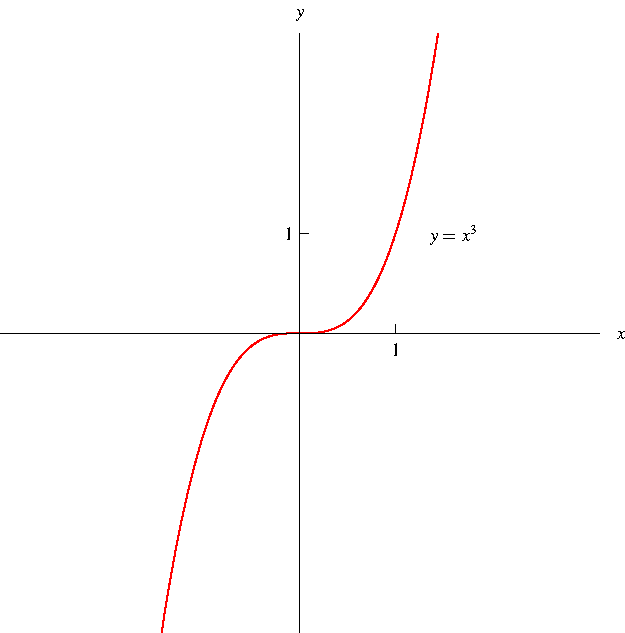
\includegraphics[width=3cm]{maxima-minima/pictures/01-02-xcubed.pdf}%
\column{.6\textwidth}
\begin{itemize}
\item<2->  Let $f(x) = x^3$.
\item<3-| alert@4-5>  Then $f'(x) = \uncover<5->{3x^2.}$
\item<3-| alert@6-7>  $f'(x) = 0$ when $x = \uncover<7->{0.}$
\item<8->  But $f$ has no local maximum or minimum at 0!
\end{itemize}
\end{columns}
\end{example}
}%

\uncover<9->{Fermat's Theorem does not say ``if $f'(c) = 0$, then $f$ has a local maximum or a local minimum at $c$.''}
\end{frame}



\begin{frame}[t]
\begin{theorem}[Fermat's Theorem]
Let $f$ be a function defined in an open interval around $c$ and such that  $f'(c)$ exists. If $f$ has a local maximum or minimum at $c$, then $f'(c) = 0$.
\end{theorem}
What does Fermat's Theorem not say?
\uncover<2->{%
\begin{example}
\begin{columns}[c]
\column{.45\textwidth}
\psset{xunit=1cm, yunit=1cm}
\begin{pspicture}(-2.5,-0.5)(2.6,2.6)
\psframe*[linecolor=white](-2.5,-0.5)(2.6,2.6)
\tiny
\psaxes[ticks=none, labels=none]{<->}(0,0)(-2.5,-0.5)(2.5,2.5)
%Function formula: (x)^{3} 
\rput(1,2){$y=|x|$} 
\psplot[linecolor=red, plotpoints=1000]{-2.5}{0}{-1 x mul  }
\psplot[linecolor=red, plotpoints=1000]{0}{2.5}{x }
\end{pspicture} 
%\ 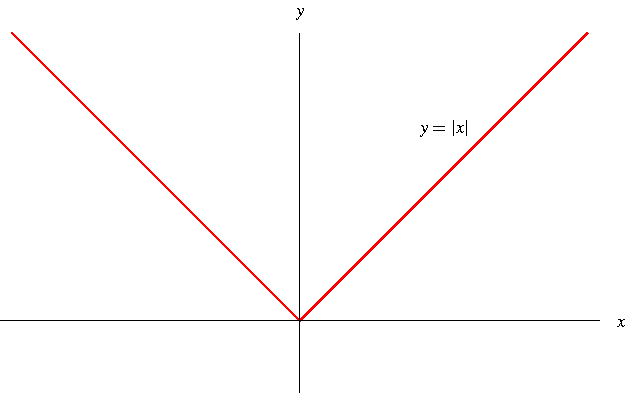
\includegraphics[width=6cm]{maxima-minima/pictures/04-01-abs.pdf}%
\column{.55\textwidth}
\begin{itemize}
\item<2->  Let $f(x) = |x|$.
\item<3-| alert@3-4>  Then $f$ has a local minimum at \uncover<4->{$0$.}
\item<5->  But $f'(0)$ doesn't exist!
\end{itemize}
\end{columns}
\end{example}
}%

\uncover<6->{Fermat's Theorem does not say ``if $f$ has a local maximum or minimum at $c$, then $f'(c)$ exists.''}
\end{frame}
% end module fermats-theorem-does-not-say
